\chapter[Percolation and the Curve \texorpdfstring{$y^2=x^3+1$}{y2 = x3 + 1}]{Percolation, Cardy's Formula and the Curve \texorpdfstring{$y^2=x^3+1$}{y2 = x3 + 1}}\label{ch:percolation}

Robert Langlands has two bodies of work that are rarely mentioned in the same breath. The first is the web of reciprocity conjectures that carries his name and that organises much of modern number theory. The second is a short burst of papers from the early 1990s, written with Philippe Pouliot and Yvan Saint Aubin, on universality and conformal invariance of crossing probabilities in two dimensional critical percolation \cite{lpps1992,lps1994}. This chapter argues that the Thorin framework of this book joins the two, and that it does so through a single random variable: the aspect ratio at which a critical rectangle stops being crossed.

The argument runs as follows. Cardy's formula for the crossing probability of a rectangle turns out to be the distribution function of a Beta$(\third,\third)$ law evaluated at the modular lambda function, and its log odds is an extended generalised gamma convolution (GGC) \cite{bondesson1992} with Thorin atoms on the lattice $\{n+\third\}$. That places percolation next to the arcsine and hyperbolic secant laws, whose atoms sit at $\{n+\tfrac12\}$ and which underlie the Pólya density of the Riemann programme. Differentiating Cardy's formula in the aspect ratio gives the density of the crossing threshold $T$, proportional to $\eta(it)^4$, and the Mellin transform of $T$ is, up to a normalising constant, the completed $L$ function of the elliptic curve $E: y^2 = x^3+1$ of conductor 36. In other words, the modularity of $E$, which is the simplest instance of Langlands reciprocity, is precisely what turns a percolation law into an $L$ function. The symmetry $T\eqd 1/T$ is the functional equation, and the characteristic function of $\log T$ is the analogue of Riemann's $\Xi$.

With that dictionary in place we study the law of $T$ itself. Its logarithm is not infinitely divisible, and $T$ is not a GGC, yet to working precision $T$ is infinitely divisible and self decomposable, which is the probabilistic form of the renormalisation fixed point that motivated the 1994 paper. Finally, the 2 sin squared lemma converts the generalised Riemann hypothesis for $E$ into a Stieltjes moment problem whose data are the cumulants of $\log T$. A Prony step on those cumulants recovers the first zero of $L(E,s)$ to twelve digits from moments of a crossing probability. The chapter ends with a set of computational problems. All numerics use mpmath, and the scripts are in the companion archive.

\section{Two programmes of Langlands}\label{perc:sec:two}

The arithmetic programme begins with a letter Langlands wrote to André Weil in January 1967 \cite{langlands1967}. Its central proposal is that algebra and analysis are two descriptions of the same objects: Galois representations on one side, automorphic forms and their $L$ functions on the other. Abelian class field theory, with Artin reciprocity as its summit, already establishes this for one dimensional representations. Langlands conjectured a non abelian generalisation, in which the transformations behind general reciprocity laws are represented by matrices and the congruences of arithmetic over finite fields are encoded in infinite dimensional representation theory. Popular accounts, including the MathWorld entry by Weisstein \cite{weisstein}, describe the result as a grand unified theory of mathematics.

The progress since then is substantial. The local conjectures for $\mathrm{GL}(n)$ over $p$ adic fields were proved by Harris and Taylor and by Henniart around 1998. Laurent Lafforgue proved the global correspondence for $\mathrm{GL}(n)$ over function fields, presented at the IAS in November 1999, and shared the 2002 Fields Medal for it. Langlands shared the 1996 Wolf Prize with Wiles, whose proof of modularity for semistable elliptic curves is itself a two dimensional case of reciprocity. Later milestones are absent from the MathWorld entry: the completion of modularity for all elliptic curves over $\mathbb{Q}$ by Breuil, Conrad, Diamond and Taylor; Ngô's proof of the fundamental lemma (Fields Medal 2010); Scholze's work on the local and geometric sides; and the 2024 proof of the unramified geometric Langlands conjecture by Gaitsgory, Raskin and their collaborators. The number field case in general remains open.

Accounts of the programme are uniformly silent on Langlands' work in mathematical physics, which is the subject of the rest of this chapter. We need only one fact from the arithmetic side, and it is the oldest kind of reciprocity for $\mathrm{GL}(2)$ over $\mathbb{Q}$: the elliptic curve $y^2 = x^3+1$ corresponds to the weight two cusp form $\eta(6\tau)^4$ of level 36. Because this curve has complex multiplication, the correspondence goes back to Deuring and Hecke and needs none of the modern machinery.

\section{Langlands, Pouliot and Saint Aubin (1994)}\label{perc:sec:lps}

The paper ``Conformal invariance in two dimensional percolation'' \cite{lps1994} appeared in the Bulletin of the AMS in 1994 (volume 30, pages 1 to 61) and grew out of Langlands' 1992 AMS Colloquium lectures. By the authors' own account nothing in it is proved. Its purpose is to state two hypotheses with complete precision and to test them by simulation on a scale that leaves little doubt. Saint Aubin, looking back in 2021 \cite{saintaubin2021}, judged it the most influential of Langlands' physics papers, because it led directly to Schramm's stochastic Loewner evolution and to Smirnov's proof of conformal invariance.

\subsection{Questions, scaling and renormalisation}

In site percolation on $\mathbb{Z}^2$ each site is open with probability $p$, independently of the others. Let $\pi^n_h(p)$ be the probability that the $n\times n$ square contains an open path from its left side to its right side. Kesten's theorem supplies a critical value $p_c\in(0,1)$: below it $\pi^n_h\to0$, above it $\pi^n_h\to1$, and at $p_c$ the $\liminf$ and $\limsup$ stay strictly inside $(0,1)$. For site percolation on the square lattice $p_c\approx0.5927460$; for bond percolation $p_c = \tfrac12$ exactly. The paper opens with three questions that Kesten's theorem leaves unanswered. Does $\pi^n_h(p_c)$ converge as $n\to\infty$? Does the slope $A_n$ of $\pi^n_h$ at $p_c$ grow like $n^{1/\nu}$ for some exponent $\nu$? And is $\nu$ universal, the same for every lattice and for sites and bonds alike? The expected answer to the last is $\nu = 4/3$.

The second part of the paper explains, for mathematicians, why physicists expect affirmative answers. Near a critical point the free energy obeys Widom's scaling relation $f(t,h) = b^{-d}f(b^{\lambda_1}t,b^{\lambda_2}h)$, with $\nu = 1/\lambda_1$. A renormalisation map $\Theta$, obtained by fusing blocks of sites into a single site, acts on a space of models, and universality classes are the stable manifolds of its unstable fixed points. Langlands' own contribution is to make this concrete through a family of finite models. One subdivides the sides of a square into $l$ intervals and records which pairs of intervals are joined by open paths; juxtaposing four such squares and composing paths defines a map $\Theta_A$, which induces a continuous map $\Theta_X$ on a finite dimensional simplex of measures. Its fixed points can be studied rigorously. The crossing probabilities are then interpreted as coordinates of the fixed point rather than of any particular model, which is the reason they should be universal.

\subsection{The two hypotheses}

An event $E$ is specified by a Jordan curve $C$, arcs $\alpha_i,\beta_i$ on $C$ that must be joined by open crossings, and arcs $\gamma_j,\delta_j$ that must not be. Write $\pi(E,M)$ for the scaling limit of the probability of $E$ under the model $M$. The group $\mathrm{GL}(2,\R)$ acts on both models and events, and the two hypotheses are stated in terms of this action.

\emph{Universality.} For any two models $M,M'$ there is $g\in\mathrm{GL}(2,\R)$ with $\pi(E,M') = \pi(E,gM)$ for every event $E$.

\emph{Conformal invariance} (suggested by Aizenman). For every model $M$ there is a complex structure $J(M)$ such that $\pi(\phi E,M) = \pi(E,M)$ for every map $\phi$ that is $J$ holomorphic or antiholomorphic inside $C$ and a homeomorphism up to the boundary.

Taken together, the hypotheses identify the image of all models in $\prod_E[0,1]$ with the quotient
\[
H(M_0)\backslash\mathrm{GL}(2,\R),
\]
which is the upper half plane, with the square lattice model $M_0$ at the point $i$. The space of critical percolation models, modulo their crossing data, is therefore the very upper half plane on which modular forms live. The authors record this without pursuing it. The rest of this chapter can be read as an attempt to pursue it.

\subsection{Exponents and Cardy's formula}

Conformal maps let the authors relate the one arm exponent, $P(r)\sim r^{-5/48}$, and the two point function, $\tau(0,z)\sim|z|^{-5/24}$, to the probability of crossing an annulus with radii $r_1<r_2$, which is approximately $(r_2/r_1)^{-5/48}$. They then give what was at the time the most accessible account of Cardy's derivation \cite{cardy1992} of the rectangle crossing probability. Percolation is treated as the $q\to1$ limit of the Potts model, so that crossing probabilities become differences of partition functions whose boundary conditions change at the four corners. The central charge is $c=0$, and the operator that changes the boundary condition is $\phi_{1,2}$, with weight $h_{1,2}=0$ in the Kac table $h_{p,q} = ((3p-2q)^2-1)/24$. Its null vector $L_{-1}^2-\tfrac23L_{-2}$ yields a hypergeometric equation and its solution,
\[
z(1-z)g''(z)+\tfrac23(1-2z)g'(z) = 0,
\qquad
\pi_h = \frac{3\Gamma(\tfrac23)}{\Gamma(\third)^2}\,z^{1/3}\,{}_2F_1\!\left(\third,\tfrac23;\tfrac43;z\right),
\]
where $z$ is the cross ratio of the four corners. On the unit disc the authors place the corners at $\pm e^{\pm i\theta_0}$, so that $z = \sin^2\theta_0$.

\subsection{Experiments and what followed}

The experiments are the substance of the paper. Rectangles containing up to $10^6$ sites, each sampled $10^6$ times, confirm Cardy's formula to about $5\times10^{-4}$. The authors then test conformal invariance in increasingly demanding settings: parallelograms at several angles and rotations, a striated model in which every lattice symmetry is broken, exterior domains, branched coverings of the disc and, at Gelfand's suggestion, compact Riemann surfaces. Each agrees with the hypotheses to within about one percent, and the authors conclude that the search for proofs can begin with moral certainty. They also observe that $\log(\pi_h/(1-\pi_h))$ is an odd function of $s = \log r$, a fact explained in Section~\ref{perc:sec:beta} below.

The proofs came within a decade. Smirnov \cite{smirnov2001} proved Cardy's formula for site percolation on the triangular lattice, and Schramm's $\mathrm{SLE}_6$ describes the scaling limit of the interfaces. The modular side emerged in parallel. Kleban and Zagier \cite{klebanzagier2003} showed that the derivative of Cardy's formula with respect to the aspect ratio is a modular form; Cardy \cite{cardy2002,cardy2006} predicted that annulus crossing probabilities are quotients of Dedekind eta functions, which was proved in 2024 \cite{sxz2024}, after Dubédat \cite{dubedat2004} had derived from $\mathrm{SLE}_6$ a differential equation that characterises the crossing probability of an annulus; and Diamantis and Kleban \cite{diamantiskleban2009} found second order modular forms in newer crossing formulas. These are the threads that the Thorin framework ties together.

\section{Cardy's formula as a Beta law with Thorin structure}\label{perc:sec:beta}

The first observation is that Cardy's hypergeometric expression is an incomplete beta function in disguise, and that the natural argument is the modular lambda function.

\begin{proposition}\label{perc:prop:beta}
Let $Z\sim\mathrm{Beta}(\third,\third)$. For a rectangle of aspect ratio $r$ (width over height),
\[
\pi_h(r) = \mathbb{P}\big(Z\le\lambda(ir)\big) = \frac{\Gamma(\tfrac23)}{\Gamma(\third)^2}\int_0^{\lambda(ir)}t^{-2/3}(1-t)^{-2/3}\,dt,
\]
where $\lambda(\tau) = \theta_2(q)^4/\theta_3(q)^4$ and $q = e^{i\pi\tau}$.
\end{proposition}
\begin{proof}
The incomplete beta identity $\int_0^z t^{a-1}(1-t)^{b-1}dt = a^{-1}z^a\,{}_2F_1(a,1-b;a+1;z)$ with $a=b=\third$ gives $3z^{1/3}{}_2F_1(\third,\tfrac23;\tfrac43;z)$, and $B(\third,\third) = \Gamma(\third)^2/\Gamma(\tfrac23)$ is Cardy's constant. The Schwarz Christoffel map from the half plane to a rectangle is an elliptic integral, and the cross ratio of the preimages of the corners is the modular lambda function at $\tau = ir$. The boundary values $\lambda\to0$ as $r\to\infty$ and $\lambda(i) = \tfrac12$ fix the orientation.
\end{proof}

\begin{remark}
The modular involution $\tau\mapsto-1/\tau$ gives $\lambda(i/r) = 1-\lambda(ir)$, and the Beta law is symmetric, $Z\eqd1-Z$. Together they give $\pi_h(1/r) = 1-\pi_h(r)$, the duality the 1994 paper checks numerically. The oddness of $\log(\pi_h/(1-\pi_h))$ in $\log r$ is simply the composition of two odd maps.
\end{remark}

Table~\ref{perc:tab:cardy} compares the Beta form with the simulated values in Table 3.2 of the 1994 paper. The agreement with the printed values of Cardy's formula is to within two units of the last digit shown, and the simulations lie within their stated error throughout.

\begin{table}[h]
\centering
\begin{tabular}{cccc}
\toprule
$r$ & simulated $\hat\pi_h$ (LPS) & Cardy as printed (LPS) & $\mathbb{P}(Z\le\lambda(ir))$ \\
\midrule
1.000 & 0.5001 & 0.5000 & 0.500000 \\
1.417 & 0.3236 & 0.3235 & 0.323408 \\
2.014 & 0.1736 & 0.1731 & 0.173091 \\
3.017 & 0.06082 & 0.06053 & 0.060551 \\
4.071 & 0.02033 & 0.02009 & 0.020080 \\
5.182 & 0.00634 & 0.00627 & 0.006273 \\
7.351 & 0.00072 & 0.00065 & 0.000647 \\
\bottomrule
\end{tabular}
\caption{Cardy's formula in Beta and theta form against the 1994 simulations.}
\label{perc:tab:cardy}
\end{table}

The disc parametrisation $z = \sin^2\theta_0$ deserves a comment, because the same substitution drives the 2 sin squared lemma \cite{polson2017}. Under $t = \sin^2\theta$ the Beta$(a,a)$ density becomes proportional to $(\sin\theta\cos\theta)^{2a-1}$ on $(0,\pi/2)$. For the arcsine law, $a = \tfrac12$, this is uniform in $\theta$; for percolation, $a = \third$, it is proportional to $(\sin2\theta)^{-1/3}$. Since the Riemann Pólya density is a scale mixture of arcsine laws, Cardy's law sits beside it as the $a = \third$ member of the symmetric Beta family, and the angle $\theta_0$ is the natural coordinate on the moduli of a quadrilateral.

The Thorin structure appears once we pass to log odds.

\begin{proposition}\label{perc:prop:thorin}
Let $U = \log\big(Z/(1-Z)\big)$ with $Z\sim\mathrm{Beta}(a,a)$. Then $U\eqd\log G_a-\log G_a'$ for independent $\mathrm{Gamma}(a)$ variables, its characteristic function is $|\Gamma(a+it)|^2/\Gamma(a)^2$, and
\[
\log\mathbb{E}\,e^{itU} = -\int_\R2\sin^2\!\Big(\frac{tx}{2}\Big)\frac{k(|x|)}{|x|}\,dx,
\]
where
\[
k(x) = \frac{e^{-ax}}{1-e^{-x}} = \sum_{n\ge0}e^{-(n+a)x} = \int_0^\infty e^{-xs}\,\mathcal{U}_a(ds),
\]
with $\mathcal{U}_a = \sum_{n\ge0}\delta_{n+a}$. Since $k$ is completely monotone, $U$ is an extended GGC in the sense of Thorin \cite{thorin1978}, with Thorin measure $\mathcal{U}_a$ on each half line.
\end{proposition}
\begin{proof}
The representation follows from $Z = G_a/(G_a+G_a')$. By Malmsten's formula for $\log\Gamma$, the Lévy measure of $\log G_a$ lives on the negative half line with density $e^{ax}/(|x|(1-e^x))$, so the symmetrised difference has density $k(|x|)/|x|$ on $\R$. Writing $\cos(tx)-1 = -2\sin^2(tx/2)$ gives the display.
\end{proof}

For percolation the Thorin atoms sit at $\third,\tfrac43,\tfrac73,\dots$. For the arcsine law they sit at $\tfrac12,\tfrac32,\dots$, and the log odds has density $(2\pi\cosh(u/2))^{-1}$ and characteristic function $1/\cosh(\pi t)$: this is the Lai Vere Jones hyperbolic secant law, and the $\cosh$ is the one in the Pólya Gamma construction. Cardy's formula can therefore be written as
\[
\pi_h(r) = \mathbb{P}\big(U\le w(\log r)\big),\qquad w(s) = \log\frac{\lambda(ie^s)}{1-\lambda(ie^s)},
\]
an extended GGC distribution function composed with an odd modular function. This is the same shape as the Riemann case, where a positive kernel built from $\theta_3$ is integrated against a law with Thorin structure.

\section{The crossing threshold and the curve \texorpdfstring{$y^2=x^3+1$}{y2 = x3 + 1}}

We now differentiate Cardy's formula in the aspect ratio. The derivative is a modular form, and that form turns out to be the one attached to an elliptic curve.

\begin{proposition}[Kleban and Zagier]\label{perc:prop:kz}
With $\eta(\tau) = q^{1/24}\prod_{n\ge1}(1-q^n)$ and $q = e^{2\pi i\tau}$,
\[
\frac{d\pi_h}{dr}(r) = -\kappa\,\eta(ir)^4,\qquad
\kappa = \frac{2^{4/3}\pi\,\Gamma(\tfrac23)}{\Gamma(\third)^2}\approx1.4936684.
\]
\end{proposition}
\begin{proof}
Use $d\lambda/d\tau = i\pi\lambda\,\theta_4^4$, so that $d\lambda/dr = -\pi\lambda\theta_4^4$ at $\tau = ir$. Differentiating Proposition~\ref{perc:prop:beta} gives $\pi_h'(r) = -\pi B(\third,\third)^{-1}\lambda^{1/3}(1-\lambda)^{-2/3}\theta_4^4$. With $\lambda = \theta_2^4/\theta_3^4$ and $1-\lambda = \theta_4^4/\theta_3^4$ this equals $-\pi B^{-1}(\theta_2\theta_3\theta_4)^{4/3}$, and Jacobi's identity $\theta_2\theta_3\theta_4 = 2\eta^3$ gives $2^{4/3}\eta^4$. We checked the identity to 25 digits at $r = 0.5, 1, 2$.
\end{proof}

Kleban and Zagier \cite{klebanzagier2003} also remark that $\pi_h(r)$ is a normalised Eichler integral of $\eta^4$, that it gives a modular parametrisation of the elliptic curve $y^2=x^3+1$, and that the constant $\kappa$ is essentially the reciprocal of one of the periods of this curve. Theorem~\ref{perc:thm:main} turns the remark into a statement about the law of the crossing threshold.

Because $\pi_h$ decreases from 1 to 0, it is a survival function, and $\kappa\,\eta(it)^4$ is a probability density on $(0,\infty)$. The corresponding random variable has a direct meaning. Fix the height at 1 and let the width $r$ grow, so that the rectangles $R_r = [0,r]\times[0,1]$ are nested. A left to right crossing of $R_{r_2}$ must meet the line $x = r_1$ before it leaves the strip, so it contains a crossing of $R_{r_1}$ for every $r_1<r_2$. The crossing event is therefore decreasing in $r$, and the crossing threshold
\[
T = \sup\{r>0: R_r\text{ has a horizontal open crossing}\}
\]
is a genuine random variable with $\mathbb{P}(T>r) = \pi_h(r)$ and density $f_T(t) = \kappa\,\eta(it)^4$ in the scaling limit (a theorem of Smirnov for site percolation on the triangular lattice, and the universality hypothesis of Section~\ref{perc:sec:lps} for the other models). We verified $\int_0^\infty f_T = 1$ numerically.

\begin{theorem}\label{perc:thm:main}
Let $E$ be the elliptic curve $y^2 = x^3+1$, of conductor $N = 36$, with $L(E,s) = \sum a_nn^{-s}$ and completed function $\Lambda(E,s) = (\sqrt N/2\pi)^s\,\Gamma(s)\,L(E,s)$. Then:
\begin{enumerate}
\item $\mathbb{E}\big[T^{s-1}\big] = \kappa\,\Lambda(E,s)$ for all $s\in\mathbb{C}$, the integral converging absolutely;
\item $\kappa = 1/\Lambda(E,1)$, equivalently
\[
L(E,1) = \frac{\Gamma(\third)^2}{3\cdot2^{4/3}\,\Gamma(\tfrac23)}\approx0.7010911;
\]
\item $T\eqd1/T$, and this is equivalent to the functional equation $\Lambda(E,s) = \Lambda(E,2-s)$ with root number $+1$;
\item the characteristic function of $\log T$ is $\Xi_E(t) := \Lambda(E,1+it)/\Lambda(E,1)$, so the Riemann hypothesis for $E$ is the statement that the characteristic function of the log crossing threshold has only real zeros.
\end{enumerate}
\end{theorem}
\begin{proof}
The form $\eta(6\tau)^4 = q\prod(1-q^{6n})^4 = q-4q^7+2q^{13}+8q^{19}-5q^{25}-\cdots$ is the newform of weight 2 and level 36 attached to $E$; we confirmed $a_p = p+1-\#E(\mathbb{F}_p)$ by point counting for all primes $p\le43$. Hence $\eta(\tau)^4 = \sum a_nq^{n/6}$, and at $\tau = it$ we have $\eta(it)^4 = \sum a_ne^{-\pi nt/3}$. Integrating term by term,
\[
\int_0^\infty t^{s-1}\eta(it)^4\,dt = \sum_na_n\,\Gamma(s)\Big(\frac{3}{\pi n}\Big)^s = \Big(\frac{6}{2\pi}\Big)^s\Gamma(s)L(E,s) = \Lambda(E,s),
\]
first for $\Re s>3/2$ and then for all $s$, since $\eta(it)^4$ decays like $e^{-\pi t/3}$ at infinity and like $t^{-2}e^{-\pi/(3t)}$ at zero by $\eta(i/t) = \sqrt t\,\eta(it)$. Multiplying by $\kappa$ gives (1). Setting $s = 1$ and using $\mathbb{E}[T^0] = 1$ gives (2); the rapidly convergent series $L(E,1) = 2\sum a_nn^{-1}e^{-2\pi n/6}$ agrees with the closed form to 25 digits. For (3), $\eta(i/t)^4 = t^2\eta(it)^4$ says $f_T(1/t)/t^2 = f_T(t)$, which is $T\eqd1/T$; in Mellin terms $\mathbb{E}[T^{s-1}] = \mathbb{E}[T^{1-s}]$, which is $\Lambda(E,s) = \Lambda(E,2-s)$. For (4) put $s = 1+it$.
\end{proof}

The parallel with the Riemann case is exact. There, a law built from $\theta_3$ (the Biane, Pitman and Yor variable \cite{bpy2001}) has Mellin transform $2\xi(s)$, and the Pólya density is the density of its logarithm. Here the Pólya kernel and its Fourier transform are
\[
\Phi_E(u) = \kappa\,e^u\,\eta(ie^u)^4,\qquad \Xi_E(t) = \int_\R\Phi_E(u)\cos(ut)\,du.
\]
$\Phi_E$ is positive, even and numerically log concave, with $(\log\Phi_E)'' = -1.30$, $-1.74$, $-2.85$ and $-7.74$ at $u = 0$, $0.5$, $1$ and $2$ respectively. Langlands reciprocity is what makes the percolation law an $L$ function; Langlands' percolation hypotheses are what make the $L$ function a probability.

Because $\Phi_E$ is explicit, positive and decays doubly exponentially, the zeros of $L(E,s)$ on the line $\Re s = 1$ can be found by direct quadrature. Locating sign changes of $\Xi_E$ gives the ordinates in Table~\ref{perc:tab:zeros}. Seventeen lie below 24, consistent with the zero counting estimate $N(T)\approx(T/\pi)\log(6T/2\pi e)\approx16.3$ plus lower order terms.

\begin{table}[h]
\centering
\begin{tabular}{cccccc}
\toprule
$k$ & $\gamma_k$ & $k$ & $\gamma_k$ & $k$ & $\gamma_k$\\
\midrule
1 & 3.443343 & 7 & 13.010560 & 13 & 19.748585\\
2 & 5.802690 & 8 & 13.996341 & 14 & 20.798454\\
3 & 7.266467 & 9 & 15.696968 & 15 & 22.189801\\
4 & 9.113425 & 10 & 16.250386 & 16 & 22.758949\\
5 & 10.174411 & 11 & 17.687326 & 17 & 23.911086\\
6 & 11.774377 & 12 & 18.858510 & & \\
\bottomrule
\end{tabular}
\caption{Real zeros of the characteristic function $\Xi_E$ of $\log T$, computed from the percolation kernel $\Phi_E$.}
\label{perc:tab:zeros}
\end{table}

\section{The reciprocal and its Thorin measure}

In the Riemann programme \cite{polson2018vdp} the Thorin structure lives on the reciprocal of $\Xi$, not on $\Xi$ itself. The same is true here. $\Xi_E$ is even and entire of order one with $\Xi_E(0) = 1$, so it has the Hadamard product $\Xi_E(t) = \prod_k(1-t^2/\rho_k^2)$ over its zeros $\rho_k$ with positive real part.

\begin{corollary}\label{perc:cor:recip}
Assume the Riemann hypothesis for $E$, so that $\rho_k = \gamma_k>0$. Then for real $y$,
\[
\frac{1}{\mathbb{E}[T^y]} = \frac{\Lambda(E,1)}{\Lambda(E,1+y)} = \frac{1}{\Xi_E(iy)} = \prod_k\frac{1}{1+y^2/\gamma_k^2} = \mathbb{E}\,e^{iyW},
\qquad W = \sum_k\frac{\varepsilon_k}{\gamma_k},
\]
with $\varepsilon_k$ independent standard Laplace variables. $W$ is a symmetric extended GGC with Thorin measure $\sum_k\delta_{\gamma_k}$ on each half line.
\end{corollary}

So the moment function $y\mapsto\mathbb{E}[T^y]$ of the crossing threshold has a reciprocal that is a characteristic function, with Thorin atoms at the zeros. This is the Thorin representation of the reciprocal Xi function transported to level 36. A necessary condition, $1/\mathbb{E}[T^y]\le1$, holds unconditionally by Jensen's inequality, since $\mathbb{E}\log T = 0$. The 2 sin squared lemma enters through Frullani's integral, $\log(1+y^2/\gamma^2) = \int_\R2\sin^2(xy/2)\,e^{-\gamma|x|}\,dx/|x|$, so that under the hypothesis
\[
-\log\mathbb{E}\,e^{iyW} = \int_\R2\sin^2\!\Big(\frac{xy}{2}\Big)\frac{k_W(|x|)}{|x|}\,dx,\qquad k_W(x) = \sum_ke^{-\gamma_kx}.
\]
This is exactly the form of Proposition~\ref{perc:prop:thorin}, with the lattice $\{n+\third\}$ replaced by the zero ordinates. The primal side admits no such representation: $\log T$ is not infinitely divisible (Theorem~\ref{perc:thm:notid} below), just as the Pólya variable of the Riemann case is not.

\section{The annulus: eta quotients and a signed measure}

Crossings of an annulus lead to a different modular object and to an instructive failure of positivity. For an annulus of modulus $L = \log(R/r)$, let $p_B$ be the probability of an open crossing and $p_{BW}$ the probability of both an open and a closed crossing. With $\tau = iL/2\pi$, Cardy's formulas \cite{cardy2002,cardy2006}, proved in 2024 \cite{sxz2024}, read
\[
p_B = \sqrt{\tfrac32}\,\frac{\eta(6\tau)\eta(\tfrac32\tau)}{\eta(2\tau)\eta(3\tau)},\qquad
p_{BW} = \sqrt3\,\frac{\eta(\tau)\eta(6\tau)^2}{\eta(3\tau)\eta(2\tau)^2}.
\]
Numerically $p_Be^{5L/48}\to\sqrt{3/2}$ and $p_{BW}e^{L/4}\to\sqrt3$, recovering the one arm exponent $5/48$ of the 1994 paper and the polychromatic two arm exponent $\tfrac14$. Taking logarithms and expanding the products, with $\sigma(m)$ the divisor sum,
\[
\log p_B(L) = \tfrac12\log\tfrac32-\frac{5L}{48}-\sum_{m\ge1}\frac{\sigma(m)}{m}\Big(e^{-\frac32mL}+e^{-6mL}-e^{-2mL}-e^{-3mL}\Big),
\]
which we checked to 20 digits at $L = 1,2,4$. This has the shape of a Lévy Khintchine exponent in $L$, with drift $5/48$ and a spectral measure on the lattice $\{\tfrac32m,2m,3m,6m\}$ weighted by divisor sums. The weights have both signs, and the next result shows that no rearrangement can remove the negative ones.

\begin{proposition}\label{perc:prop:annulus}
$p_B$ is not the Laplace transform of a positive measure on $[0,\infty)$; the signed measure above cannot be replaced by a positive one.
\end{proposition}
\begin{proof}
By the modular dual form, $1-p_B(L) = O(e^{-c/L})$ as $L\to0$; numerically $1-p_B(0.2)\approx5\times10^{-15}$. If $p_B(L) = \int e^{-Lx}\mu(dx)$ with $\mu\ge0$ of mass one and not a point mass at zero, then $1-p_B(L) = \int(1-e^{-Lx})\mu(dx)\ge c'L$ for small $L$, a contradiction. A point mass at zero would make $p_B\equiv1$.
\end{proof}

The reciprocal Xi function meets the same obstruction: a natural exponential representation exists, but only with a signed measure, and the real question is which transform of it is positive.

\section{Structure of the threshold law}\label{perc:sec:progress}

Three structural questions about $T$ arise at once. Is it a GGC? Is $\log T$ infinitely divisible? Can the Thorin measure of the reciprocal be computed from moments of $T$? This section answers the first two in the negative, shows that a weaker structure survives, and gives a working method for the third. Section~\ref{perc:sec:sin2} then turns that method into a criterion.

\subsection{Two negative results}\label{perc:sec:notggc}

The first negative result is immediate from Theorem~\ref{perc:thm:main}.

\begin{theorem}\label{perc:thm:notid}
$\log T$ is not infinitely divisible; in particular it is not an extended GGC.
\end{theorem}
\begin{proof}
The characteristic function of an infinitely divisible law has no real zeros. The characteristic function of $\log T$ is $\Xi_E$, which vanishes at the ordinate of every zero of $L(E,s)$ on the line $\Re s = 1$. Such zeros exist: the first is at $\gamma_1 = 3.443343\ldots$ (Table~\ref{perc:tab:zeros}), where $\Xi_E$ changes sign, and one is all that the proof needs. There are in fact infinitely many: Rezvyakova \cite{rezvyakova2010} proved that a positive proportion of the zeros of the $L$ function of a Hecke eigenform for $\Gamma_0(D)$ lie on the critical line, which extends Hafner's theorem \cite{hafner1983} for the full modular group.
\end{proof}

This is not a defect of the example but the design of the programme. As with the Pólya variable of the Riemann case, the primal law cannot carry a Lévy or Thorin representation, and the reciprocal is where the Thorin structure must live.

The second negative result concerns $T$ itself and needs the analytic continuation of its Laplace transform, which is a series in the Fourier coefficients of $E$.

\begin{lemma}\label{perc:lem:lap}
The Laplace transform $\varphi(s) = \mathbb{E}\,e^{-sT}$ extends to a meromorphic function on $\mathbb{C}$,
\[
\varphi(s) = \int_0^{t_0}e^{-st}f_T(t)\,dt+\kappa\sum_{n\ge1}a_n\,\frac{e^{-(s+\pi n/3)t_0}}{s+\pi n/3}
\qquad(\text{any }t_0>0),
\]
with simple poles at $s = -\pi n/3$ for each $n$ with $a_n\ne0$ ($n = 1,7,13,19,25,\dots$) and residue $\kappa a_n$. Formally $\varphi(s) = \kappa\sum_na_n/(s+\pi n/3)$.
\end{lemma}
\begin{proof}
Split the Laplace integral at $t_0$ and insert $f_T(t) = \kappa\sum a_ne^{-\pi nt/3}$ on $[t_0,\infty)$. Since $a_n$ grows at most polynomially, the series converges absolutely and locally uniformly away from the poles. With $t_0 = 0.2$ the formula reproduces $\varphi(1)$ and $\varphi(-\tfrac12)$, computed directly, to fifteen or more digits.
\end{proof}

\begin{theorem}\label{perc:thm:notggc}
$T$ is not a generalised gamma convolution. Consequently its density $\kappa\,\eta(it)^4$ is not hyperbolically completely monotone.
\end{theorem}
\begin{proof}
The residues at the consecutive poles $-13\pi/3$ and $-19\pi/3$ are $2\kappa$ and $8\kappa$, and no $n$ strictly between 13 and 19 has $a_n\ne0$. Just to the right of $-19\pi/3$, $\varphi\to+\infty$; just to the left of $-13\pi/3$, $\varphi\to-\infty$. Since $\varphi$ is real and continuous on the open gap, it has a zero $s_*$ there, numerically $s_* = -15.0217943\ldots$.

If $T$ were a GGC, then $-\varphi'/\varphi = a+\int U(dt)/(s+t)$ would be a Stieltjes function with $U\ge0$. Here $-\varphi'/\varphi$ is meromorphic, so Stieltjes inversion identifies $U$ with the point masses given by its residues on the negative axis. At the zero $s_*$ that residue is $-1$, contradicting $U\ge0$. Since HCM laws are GGC, the density is not HCM.
\end{proof}

A direct test of hyperbolic complete monotonicity confirms this independently and shows how subtle the failure is. For $u = 1$ the function $g(w) = f_T(uv)f_T(u/v)$, with $w = v+1/v$, has $(-1)^4g^{(4)}(2.2) = -0.59$ and $(-1)^5g^{(5)}(3) = -0.012$, values that are stable under changes of the differentiation step. At $u = 0.3,0.6,2,3.5$, by contrast, the first six derivatives all have the right sign.

\subsection{Infinite divisibility and self decomposability}

Although $T$ falls outside the Thorin class, a weaker structure survives. The ratio $-\varphi'/\varphi$ is positive on $(0,\infty)$ and decays like $\sqrt{\pi/(3s)}$, as the behaviour $f_T(t)\sim\kappa t^{-2}e^{-\pi/(3t)}$ at the origin predicts. Inverting it numerically (de Hoog's method at 40 digits) gives
\[
-\frac{\varphi'(s)}{\varphi(s)} = \int_0^\infty e^{-sx}\,m(x)\,dx,
\qquad
m(x)\overset{\text{formally}}{=}\sum_{a_n\ne0}e^{-\pi nx/3}-\sum_{\varphi(z)=0}e^{zx}.
\]
$T$ is infinitely divisible exactly when $m\ge0$, in which case its Lévy measure is $m(x)\,dx/x$, and it is self decomposable exactly when $m$ is in addition nonincreasing.

\begin{proposition}[numerical]\label{perc:prop:sd}
On a grid of 39 points in $[0.02,5.9]$, $m(x)$ is positive (minimum $0.0021$) and strictly decreasing, and $m(x)e^{\pi x/3}\to1$ (to $10^{-8}$ by $x = 3$), reflecting the leading pole at $n = 1$. To working precision, therefore, $T$ is infinitely divisible and self decomposable. It is not a GGC because $m$ is not completely monotone: the zeros of $\varphi$ enter with negative weight.
\end{proposition}

\begin{figure}[h]
\centering
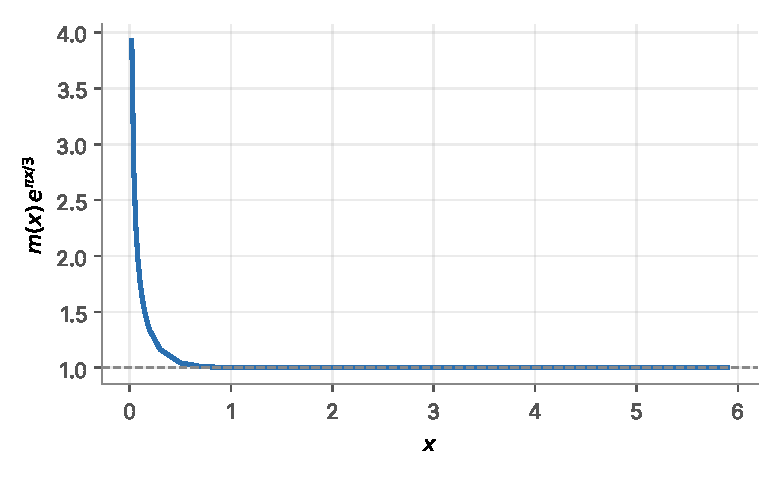
\includegraphics[width=\textwidth]{figs/perc_fig_m.pdf}
\caption{The normalised Lévy function $m(x)e^{\pi x/3}$ of $T$. It is positive, decreasing and tends to 1.}
\label{perc:fig:m}
\end{figure}

The pole and zero formula explains why positivity survives. Each real zero $z$ that we found lies in a gap $(-\pi n_{j+1}/3,-\pi n_j/3)$ between poles and pairs with the pole to its right, contributing $e^{-\pi n_jx/3}-e^{-|z|x}>0$. Seventeen real zeros appear among the 33 poles up to $n = 229$, and they occur exactly in the 17 gaps where consecutive residues share a sign, one in each. The argument principle on the box $[-238.8,1]\times[-40,40]$, which contains the 32 poles with $n\le223$, counts 23 zeros in all; the remaining six are complex or closely spaced real pairs, and Proposition~\ref{perc:prop:sd} indicates that they are dominated.

Self decomposability is the renormalisation statement of the 1994 paper in probabilistic form. For every $c\in(0,1)$ we have $T\eqd cT+T_c$ with $T_c$ independent of $T$, so the crossing threshold is a fixed point of the map that rescales and adds an independent block. Since $T\eqd1/T$, the same holds for $1/T$. The Thorin class is one step too small for the threshold; the self decomposable class is its natural home.

\subsection{From moments to zeros}\label{perc:sec:cum}

The third question asks whether the Thorin measure of the reciprocal, which under the hypothesis is the zero measure $\sum\delta_{\gamma_k}$, can be computed from the law of $T$. It can, through the cumulants of $X = \log T$. Write $K_X(y) = \log\mathbb{E}\,e^{yX} = \log\big(\Lambda(E,1+y)/\Lambda(E,1)\big)$ for the cumulant generating function.

\begin{proposition}\label{perc:prop:cum}
Let $Z_m = \sum_\rho\rho^{-2m}$, the sum over zeros of $\Xi_E$ with $\Re\rho>0$; there are none on the imaginary axis, since $\Xi_E(iy) = \mathbb{E}\,e^{-yX}>0$. Then, unconditionally, the odd cumulants of $X$ vanish and
\[
\kappa_{2m}(X) = (-1)^{m+1}\,\frac{(2m)!}{m}\,Z_m.
\]
The candidate reciprocal law $W$ of Corollary~\ref{perc:cor:recip} has $\varphi_W(y) = e^{-K_X(y)}$ and $\kappa_{2m}(W) = (-1)^{m+1}\kappa_{2m}(X)$; in particular $\mathrm{Var}(W) = \mathrm{Var}(\log T) = 2Z_1$. Under the Riemann hypothesis for $E$, $Z_m = \sum_k\gamma_k^{-2m}>0$ for every $m$ and $Z_m^{-1/(2m)}\uparrow\gamma_1$.
\end{proposition}
\begin{proof}
Take logarithms in $\Xi_E(t) = \prod(1-t^2/\rho^2)$ and expand $\log(1-u) = -\sum u^m/m$. The statement about $W$ is the Wick rotation $t\mapsto iy$ applied to the same series.
\end{proof}

The Thorin measure of the reciprocal is thus read off the cumulants of the crossing threshold with alternating signs, which is the 2 sin squared lemma at the level of cumulants. Table~\ref{perc:tab:Zm} computes $Z_m$ from eight even moments of $\log T$, obtained by quadrature of $\Phi_E$ at 30 digits, and compares them with the sums over the seventeen zeros of Table~\ref{perc:tab:zeros}.

\begin{table}[h]
\centering
\begin{tabular}{cccc}
\toprule
$m$ & $Z_m$ from cumulants of $\log T$ & $\sum_{k\le17}\gamma_k^{-2m}$ & $Z_m^{-1/(2m)}$ \\
\midrule
1 & 0.251339427650 & 0.197344721657 & 1.99466 \\
2 & 8.80236407504$\times10^{-3}$ & 8.77716934058$\times10^{-3}$ & 3.26475 \\
3 & 6.36554168387$\times10^{-4}$ & 6.36529963503$\times10^{-4}$ & 3.40953 \\
4 & 5.15425327124$\times10^{-5}$ & 5.15425044654$\times10^{-5}$ & 3.43542 \\
5 & 4.29363900865$\times10^{-6}$ & 4.29363897255$\times10^{-6}$ & 3.44126 \\
6 & 3.60681298867$\times10^{-7}$ & 3.60681298818$\times10^{-7}$ & 3.44276 \\
7 & 3.03794521992$\times10^{-8}$ & 3.03794521992$\times10^{-8}$ & 3.44317 \\
8 & 2.56106278207$\times10^{-9}$ & 2.56106278206$\times10^{-9}$ & 3.44329 \\
\bottomrule
\end{tabular}
\caption{Zero sums of $L(E,s)$ recovered from the crossing threshold. The gap at $m = 1$ is the slowly convergent tail of zeros beyond 24.}
\label{perc:tab:Zm}
\end{table}

Every $Z_m$ is positive, and $Z_m^{-1/(2m)}$ increases towards $\gamma_1 = 3.443343$. The agreement with the zero sums improves rapidly with $m$. At $m = 8$ the last printed digits of the two columns differ only through rounding: before rounding the discrepancy is $1.0\times10^{-22}$, which is the expected contribution of the zeros beyond the table ($24.5^{-16}\approx6\times10^{-23}$). Moments of a crossing probability therefore determine the low lying zeros of an elliptic curve $L$ function. This is the computational path of the Thorin Xi programme, carried out at level 36.

The candidate reciprocal law can also be examined directly. Corollary~\ref{perc:cor:recip} requires $y\mapsto1/\mathbb{E}[T^y]$ to be positive definite, so we computed the candidate density
\[
p_W(x) = \frac1\pi\int_0^\infty\frac{\cos(xy)}{\mathbb{E}[T^y]}\,dy
\]
by the trapezoid rule. The rule converges spectrally here because the integrand is even and $1/\mathbb{E}[T^y]$ decays faster than exponentially, reaching $7\times10^{-19}$ at $y = 20$. The resulting density has total mass $1.0000000$ and is positive on $[0,8]$, with smallest value $1.6\times10^{-11}$ at $x = 8$. Its tail decays at the local rates $3.254,3.374,3.420,3.436,3.4418,3.4432$ over $[2,6]$, converging to $\gamma_1$ as they must, since the nearest singularity of $1/\Xi_E(iy)$ is at $y = \pm i\gamma_1$. Figure~\ref{perc:fig:pW} shows the density; its slope reads off the first zero of $L(E,s)$.

\begin{figure}[h]
\centering
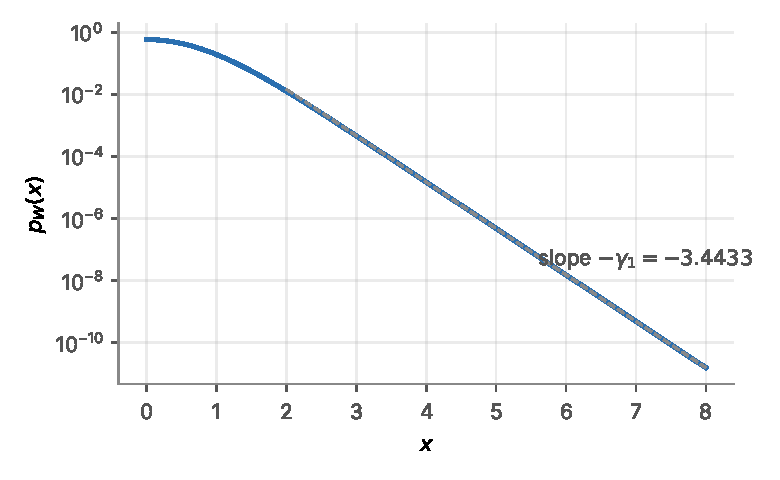
\includegraphics[width=\textwidth]{figs/perc_fig_pW.pdf}
\caption{The reciprocal density $p_W$ on a log scale. The dashed line has slope $-\gamma_1$, the first zero of $L(E,s)$.}
\label{perc:fig:pW}
\end{figure}

\section{What the 2 sin squared lemma buys}\label{perc:sec:sin2}

The 2 sin squared lemma carries the Lévy measure of a primal function to the Thorin measure of its reciprocal. In this chapter it does real work: it converts the zero question for $L(E,s)$ into a Stieltjes moment problem whose data are the cumulants of the crossing threshold. That yields both an equivalent form of GRH for $E$ and an algorithm that recovers the zeros.

\subsection{The lemma in this setting}

For a symmetric law $W$ with Lévy density $k(|x|)/|x|$, where $k(x) = \int_0^\infty e^{-xt}\,U(dt)$, the identity $1-\cos = 2\sin^2$ and Frullani's integral give
\[
-\log\mathbb{E}\,e^{iyW} = \int_\R2\sin^2\!\Big(\frac{xy}{2}\Big)\frac{k(|x|)}{|x|}\,dx = \int_0^\infty\log\Big(1+\frac{y^2}{t^2}\Big)\,U(dt).
\]
The middle expression is the Lévy side and the right side is the Thorin side. We apply this to $K_X(y) = \log\mathbb{E}\,e^{yX}$ with $X = \log T$, which is the candidate $-\log\varphi_W$ of Corollary~\ref{perc:cor:recip}. The Hadamard product gives, unconditionally,
\[
K_X(y) = \sum_\rho\log\Big(1+\frac{y^2}{\rho^2}\Big),
\]
so the lemma identifies the candidate Thorin measure as the zero counting measure $\sum_\rho\delta_\rho$. This is a positive measure on $(0,\infty)$ exactly when every $\rho$ is real. Differentiating once and setting $u = y^2$ linearises the problem:
\begin{gather*}
G(u) := \frac{K_X'(\sqrt u)}{2\sqrt u} = \sum_\rho\frac{1}{u+\rho^2} = \sum_{m\ge1}(-u)^{m-1}Z_m,\\
Z_m = (-1)^{m+1}\frac{m\,\kappa_{2m}(\log T)}{(2m)!}.
\end{gather*}
The function $G$ is computable from the law of $T$ alone, and its Taylor coefficients are the zero sums of Proposition~\ref{perc:prop:cum}.

\subsection{A GRH criterion in percolation cumulants}

\begin{theorem}\label{perc:thm:crit}
The following are equivalent.
\begin{enumerate}
\item The Riemann hypothesis holds for $L(E,s)$, $E: y^2 = x^3+1$.
\item $y\mapsto1/\mathbb{E}[T^y]$ is the characteristic function of a symmetric extended GGC; that is, the Thorin measure produced by the 2 sin squared lemma is positive.
\item $G$ is a Stieltjes function.
\item For every $n$ the Hankel matrix $H_n = [Z_{i+j+1}]_{i,j=0}^{n-1}$, built from the even cumulants of $\log T$, is positive semidefinite.
\end{enumerate}
\end{theorem}
\begin{proof}
That (1) implies (2) is Corollary~\ref{perc:cor:recip}. If (2) holds with Thorin measure $U\ge0$, the display above gives $\sum_\rho\log(1+y^2/\rho^2) = \int\log(1+y^2/t^2)\,U(dt)$. Both sides are meromorphic in $u = y^2$ after one differentiation, and matching poles forces $U = \sum\delta_\rho$ with every $\rho^2>0$, which is (3). Next, $G$ is meromorphic with poles at $u = -\rho^2$ and residues equal to the multiplicities. A Stieltjes function has poles only on the negative axis with positive residues, so (3) forces $\rho^2>0$. There are no zeros on the imaginary axis because $\Xi_E(iy) = \mathbb{E}\,e^{-yX}>0$, so each $\rho$ is real, which is (1).

For (1) implies (4), put $w_\rho = \rho^{-2}>0$. Then $Z_{k+1} = \int w^k\,\nu(dw)$ for the positive measure $\nu = \sum_\rho w_\rho\delta_{w_\rho}$, and Hankel matrices of moments of a positive measure are positive semidefinite. For (4) implies (1), positivity of every $H_n$ gives, by Hamburger's theorem, a positive measure $\nu$ with moments $Z_{k+1}$. Let $\rho_1$ be a zero of least modulus. Since $|Z_m|\le\sum|\rho|^{-2m}\le C|\rho_1|^{-2m}$, $\nu$ is supported in $[-|\rho_1|^{-2},|\rho_1|^{-2}]$ and is determinate. Its Cauchy transform $\int\nu(dw)/(z-w) = \sum_kZ_{k+1}z^{-k-1} = \sum_\rho w_\rho/(z-w_\rho)$ agrees with this meromorphic function near infinity, hence everywhere. The Cauchy transform of a positive measure on $\R$ has only real singularities, with positive residues at atoms, so every $w_\rho = \rho^{-2}$ is real and positive and every $\rho$ is real.
\end{proof}

Theorem~\ref{perc:thm:crit} is the percolation form of the moment criteria for RH in the style of Li and Keiper. What distinguishes it is that the data are moments of a probability law with a physical meaning, the aspect ratio at which a critical rectangle stops being crossed. There is also an equivalent heat trace form,
\[
G(u) = \int_0^\infty e^{-uv}\,h(v)\,dv,\qquad h(v) = \sum_\rho e^{-\rho^2v},
\]
so that GRH for $E$ holds exactly when the heat trace $h$ over the zeros, computed from percolation, is completely monotone. This is the level 36 version of the heat trace approach to RH developed elsewhere in this book.

\subsection{Hankel positivity and Prony recovery of the zeros}

Eighteen even moments of $\log T$, computed at 80 digits by quadrature of $\Phi_E$, give $Z_1,\dots,Z_{18}$, and the first eight Hankel determinants are all positive:
\[
\begin{array}{cccc}
\Delta_1 = 0.2513 & \Delta_2 = 8.25\times10^{-5} & \Delta_3 = 6.22\times10^{-12} & \Delta_4 = 3.41\times10^{-23}\\
\Delta_5 = 8.55\times10^{-39} & \Delta_6 = 5.80\times10^{-59} & \Delta_7 = 4.83\times10^{-84} & \Delta_8 = 3.82\times10^{-114}
\end{array}
\]
The determinants decrease super exponentially, so each new one needs substantially more working precision than the last. This is the practical limit of the criterion: a finite computation certifies the low lying zeros, not GRH.

The lemma also supplies an algorithm. The Thorin atoms $w_\rho = \rho^{-2}$ are the nodes of a Gauss type quadrature for the moments $Z_m$, so a Prony step recovers them. Solving the $n$ atom Hankel system on the top moments $Z_{18-2n+1},\dots,Z_{18}$ and taking $\gamma = w^{-1/2}$ gives Table~\ref{perc:tab:prony}.

\begin{table}[h]
\centering
\begin{tabular}{ccccc}
\toprule
atoms $n$ & $\gamma_1$ & $\gamma_2$ & $\gamma_3$ & $\gamma_4$\\
\midrule
2 & 3.44334336792 & 5.80445751428 & & \\
4 & 3.44334336791 & 5.80268979301 & 7.26707176506 & 9.31510586734\\
6 & 3.44334336791 & 5.80268955576 & 7.26648441131 & 9.13983526637\\
8 & 3.44334336791 & 5.80268955297 & 7.26647026339 & 9.12131542682\\
\midrule
direct & 3.44334336791 & 5.80268955255 & 7.26646731082 & 9.11342494550\\
\bottomrule
\end{tabular}
\caption{Zeros of $L(E,s)$ recovered as Thorin atoms from cumulants of the crossing threshold, against direct computation from $\Xi_E$.}
\label{perc:tab:prony}
\end{table}

The first zero is recovered to twelve digits, the second to nine and the third to five, and every recovered atom is real and positive, as Theorem~\ref{perc:thm:crit} requires. The lemma does not help on the primal side: $\log T$ has no Lévy measure (Theorem~\ref{perc:thm:notid}) and $T$ is not symmetric, so the lemma is used exactly once, on the reciprocal. That is the same division of labour as in the treatment of the reciprocal Xi function.

\section{Renormalisation and the Thorin class}

We return to the question that motivated the 1994 paper: why should crossing probabilities be universal? Langlands' answer was that they are coordinates of a fixed point of renormalisation, and the results of this chapter let us say what kind of fixed point.

The Thorin class has exactly the closure properties a renormalisation map requires. GGC laws are closed under convolution, scaling and weak limits, and every GGC is self decomposable, so that $X\eqd cX+X_c$ for each $c\in(0,1)$. That identity is a fixed point equation for the map that rescales by $c$ and adds an independent block, which is a probabilistic shadow of the block fusion map $\Theta$. Widom's relation $f(t,h) = b^{-d}f(b^{\lambda_1}t,b^{\lambda_2}h)$ is a homogeneity statement of the same kind as the dilation $\mathcal{U}(dt)\mapsto\mathcal{U}(b\,dt)$ of a Thorin measure.

Section~\ref{perc:sec:progress} sharpens this picture in two directions. The crossing log odds $U$ of Proposition~\ref{perc:prop:thorin} is an extended GGC, so the conformally invariant crossing data live in the Thorin class. The crossing threshold $T$, by contrast, is self decomposable but not a GGC, so its fixed point property holds only in the larger class. A concrete version of Langlands' finite model programme in this language would let $\Theta_X$ act on Lévy functions $m(x)$ rather than on simplices of crossing configurations, and ask whether the crossing data of Section~\ref{perc:sec:beta} is a fixed point.

\section{Open computational problems}\label{perc:sec:problems}

We close with problems that are open and largely computational. The scripts in the chapter's companion archive compute every quantity used above and are the natural starting point for each.

\begin{compproblem}[Lévy function of the threshold]
Prove Proposition~\ref{perc:prop:sd}: show that $m(x) = \sum_{a_n\ne0}e^{-\pi nx/3}-\sum_{\varphi(z)=0}e^{zx}$ is positive and nonincreasing. A natural route is an interlacing theorem for the zeros of $\kappa\sum a_n/(s+\pi n/3)$ against its poles, controlling the complex zeros through the CM structure of the coefficients $a_n$ (the curve has complex multiplication by $\mathbb{Z}[\omega]$).
\end{compproblem}

\begin{compproblem}[positive definiteness and complex zeros]
Theorem~\ref{perc:thm:crit} shows that GRH for $E$ is equivalent to $1/\mathbb{E}[T^y]$ being the characteristic function of a symmetric extended GGC. Is mere positive definiteness enough? A complex zero pair contributes a factor $\big((1+y^2/\rho^2)(1+y^2/\bar\rho^2)\big)^{-1}$, which is the characteristic function of a signed measure; decide whether the full product can nonetheless be positive definite.
\end{compproblem}

\begin{compproblem}[other crossing events]
Kleban and Zagier treat $\pi_{hv}$ and Watts' formula, and Diamantis and Kleban find second order modular forms. For each event, identify the Mellin transform of the associated threshold, determine which $L$ functions or Eichler type integrals arise, and decide whether the threshold is self decomposable.
\end{compproblem}

\begin{compproblem}[annulus thresholds]
The modulus at which an annulus stops being crossed has survival function $p_B(L)$. Its Laplace transform is again meromorphic, with poles at the exponents $(5+24j)/48$ of the eta quotient expansion, so the method of Section~\ref{perc:sec:notggc} applies directly. Decide whether this threshold is a GGC or self decomposable, and identify its Mellin transform.
\end{compproblem}

\begin{compproblem}[universality on the upper half plane]
The 1994 paper identifies critical models, up to crossing data, with $H(M_0)\backslash\mathrm{GL}(2,\R)$. Does the family of thresholds $T_z$ for parallelograms of modulus $z$ define a Mellin family indexed by the upper half plane, and does Hecke theory act on it?
\end{compproblem}

\section{Numerical methods}\label{perc:sec:numerics}

All computations use mpmath at between 20 and 80 digits.
\begin{itemize}
\item The lambda function comes from Jacobi theta functions, and Cardy's formula from the regularised incomplete beta function.
\item $\eta(it)$ comes from the $q$ Pochhammer symbol, using the inversion $\eta(it) = \eta(i/t)/\sqrt t$ for $t<1$.
\item Fourier and Mellin integrals use tanh sinh quadrature.
\item The coefficients of $\eta(6\tau)^4$ come from direct expansion of the product to $q^{1500}$, and $a_p$ from brute force point counting.
\item The continuation of $\varphi$ uses Lemma~\ref{perc:lem:lap} with $t_0 = 0.2$ and Gauss Legendre nodes. Real zeros come from sign changes followed by root polishing, and the total zero count from the argument principle.
\item Laplace inversion uses de Hoog's method.
\item HCM derivatives were taken by numerical differentiation at 40 digits, with two step sizes.
\end{itemize}
